\documentclass[11pt]{report}
\usepackage{tikz}
\usetikzlibrary{fit,positioning}
\begin{document}
\begin{figure}
\centering
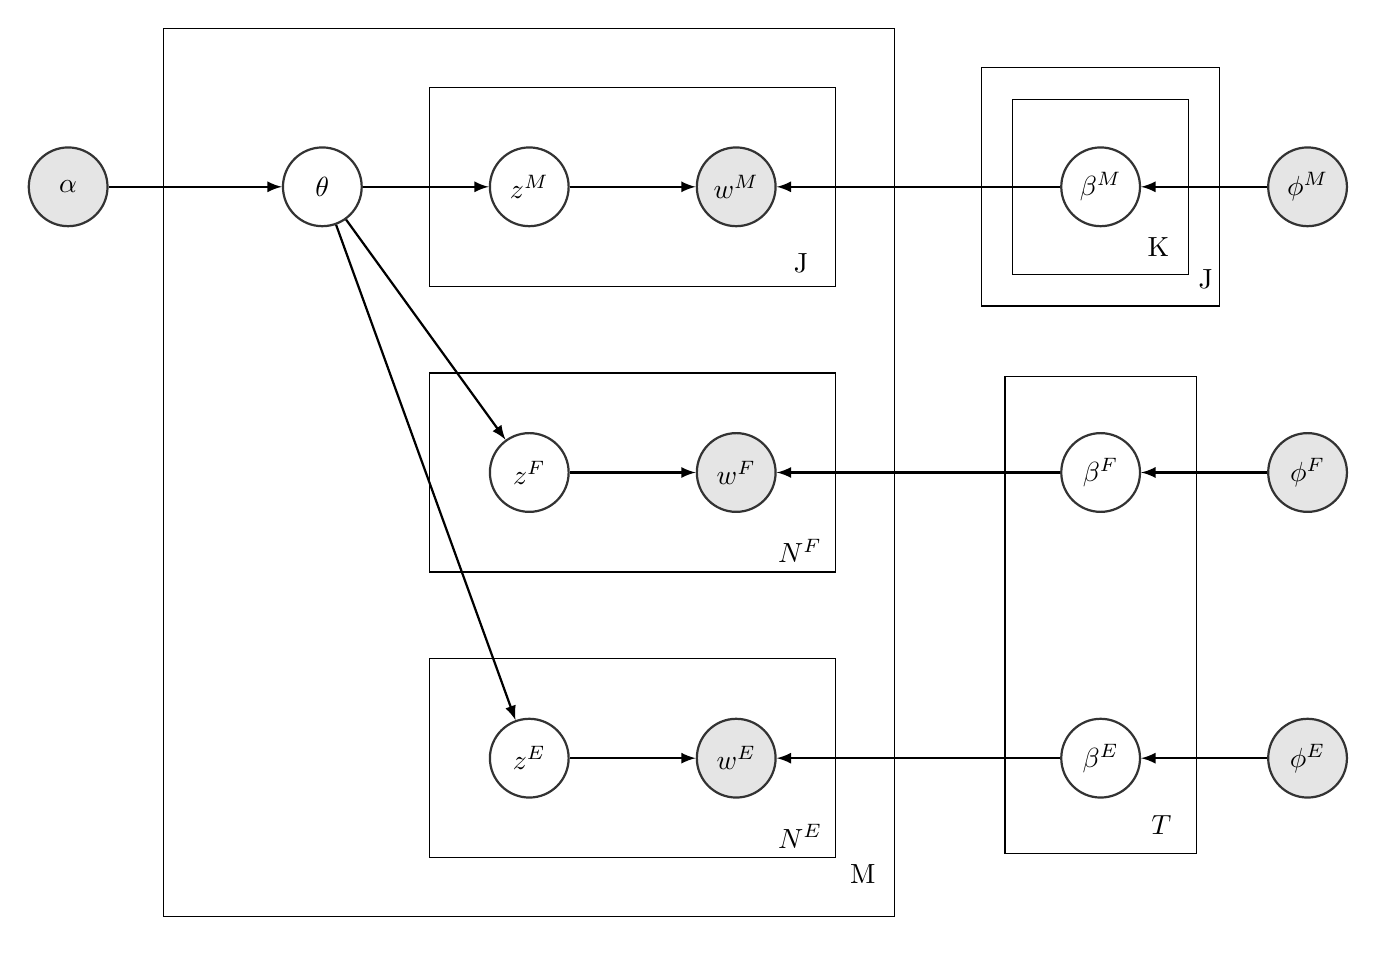
\begin{tikzpicture}
\tikzstyle{main}=[circle, minimum size = 10mm, thick, draw =black!80, node distance = 16mm]
\tikzstyle{connect}=[-latex, thick]
\tikzstyle{box}=[rectangle, draw=black!100]

    % 节点的定义,图中的圆
  \node[main, fill = black!10] (alpha)  { $\alpha$};
  \node[main] (theta) [right=of alpha, xshift=0.6cm] { $\theta$};
  \node[main] (zm) [right= of theta]{$z^M$ };
  \node[main, fill = black!10] (wm) [right= of zm] {$w^M$};
  \node[main] (zf) [below=of zm, yshift= -1cm] {$z^F$ };
  \node[main] (ze) [below=of zf, yshift= -1cm] {$z^E$ };
  \node[main, fill = black!10] (wf) [right=of zf] { $w^F$};
  \node[main, fill = black!10] (we) [right=of ze] { $w^E$};
  \node[main] (beta_f) [right=of wf, xshift = 2cm] {$\beta^F$ };
  \node[main] (beta_e) [right=of we, xshift = 2cm] { $\beta^E$};
  \node[main] (beta_m)[right = of wm, xshift = 2cm]{$\beta^M$};
  \node[main, fill = black!10] (phi_f) [right=of beta_f] {$\phi^F$ };
  \node[main, fill = black!10] (phi_e) [right=of beta_e] {$\phi^E$ };
  \node[main, fill = black!10] (phi_m)[right = of beta_m]{$\phi^M$};

    % 边的定义,
  \path (alpha) edge [connect] (theta)
        (theta) edge [connect] (zm)
        (theta) edge [connect] (zf)
        (theta) edge [connect] (ze)
        (zf) edge [connect] (wf)
        (ze) edge [connect] (we)
        (zm) edge [connect] (wm)
        (beta_f) edge [connect] (wf)
        (beta_e) edge [connect] (we)
        (beta_m)edge[connect](wm)
        (phi_f) edge [connect] (beta_f)
        (phi_e) edge [connect] (beta_e)
        (phi_m) edge [connect] (beta_m);

    % 节点的定义,图中的矩形
  \node[rectangle, inner sep=2mm, fit= (zf) (wf),label=below right:$N^F$, xshift = 1cm] {};
  \node[rectangle, inner sep=7.5mm,draw=black!100, fit= (zf) (wf)] {};
  \node[rectangle, inner sep=2mm, fit= (ze) (we),label=below right:$N^E$, xshift = 1cm] {};
  \node[rectangle, inner sep=7.5mm,draw=black!100, fit= (ze) (we)] {};
  \node[rectangle, inner sep=2mm, fit= (zf) (wf)(ze)(we),label=below right:M, xshift= 0.6cm, yshift = -1cm] {};
  \node[rectangle, inner sep=15mm, draw=black!100, fit = (theta) (zf) (wf)(ze)(we)] {};]
  \node[rectangle, inner sep = 2mm, fit = (zm) (wm), label=below right: J, xshift = 1.2cm]{};
  \node[rectangle, inner sep = 7.5mm, draw = black!100, fit = (zm)(wm)]{};

 \node[rectangle, inner sep = 1mm, fit = (beta_m), label = below right : J, xshift = 0.5cm, yshift=-0.3cm]{};
 \node[rectangle, inner sep = 10mm, draw = black!100, fit = (beta_m)]{};
 
  \node[rectangle, inner sep = 1mm, fit = (beta_m), label = below right: K, xshift = -0.15cm, yshift=0.1cm]{};
 \node[rectangle, inner sep = 6mm, draw = black!100, fit = (beta_m)]{};

  \node[rectangle, inner sep = 1mm, fit = (beta_f)(beta_e), label = below right: $T$, xshift = -0.1cm, yshift=-1.8cm]{};
  \node[rectangle, inner sep = 7mm, draw=black!100, fit = (beta_f)(beta_e)]{};

\end{tikzpicture}
\end{figure}
\end{document}
%note - compiled with pdflatex
